\documentclass[preprint]{elsarticle}
\usepackage[margin=0.5in]{geometry}
\usepackage{amsmath}
\usepackage{amsfonts} % \mathbb
\usepackage{amssymb}  % \therefore
\usepackage{algorithm}
\usepackage{algorithmic}
\usepackage{lineno,hyperref}

\bibliographystyle{elsarticle-num}
\begin{document}
\begin{frontmatter}

\title{Envelope Estimation using Geometric Properties of a Discrete Real Signal}

\cortext[cor1]{Corresponding author}
\address{Department of Production Engineering, Universidade Federal Fluminense, Rua Passo da Pátria, 156, Campus Praia Vermelha, Bloco D - sala 309, São Domingos, Niterói, RJ, Brasil, CEP: 24.210-240}

\author{Carlos Henrique Tarjano Santos\corref{cor1}}
\ead{carlostarjano@id.uff.br}

\author{Valdecy Pereira}

\begin{abstract} 
Despite being an elusive concept, the temporal amplitude envelope of a signal is essential for its complete characterization, being the primary information-carrying medium in spoken voice and telecommunications, for example. Envelope detection techniques have applications in areas like medicine, sound classification and synthesis, seismology, and speech recognition. Nevertheless, a general approach to envelope detection doesn't exist, as most methods involve manual intervention, in the form of filter design, smoothing, and other specific design choices based on prior knowledge of the signals under investigation. To address this problem, we propose an algorithm that uses characteristics of a signal to estimate its envelope, eliminating the necessity of parameter tuning. The method draws inspiration from geometric concepts; the discrete signal is mapped to a set of points in the Cartesian plane, where a new measure of discrete curvature is used to identify the samples that are part of the envelope. Due to its geometric nature, the method can optionally generate the superior and inferior envelopes of a given wave. The algorithm compares favorably with classic envelope detection techniques based on smoothing, filtering, and the Hilbert Transform, besides being physically plausible. We provide visualizations of the envelope extracted for various real-world signals with very diverse characteristics, such as voice, spoken and sang, and pitched and unpitched musical instruments, and discuss some approaches to objectively assess the quality of the obtained envelopes. An optimized implementation is available via the Python Package Index (PyPI); interactive visualizations and source code are available at the accompanying repository.
\end{abstract}

\begin{keyword}
  DSP \sep alpha shapes \sep envelope detection \sep discrete curvature estimation \sep demodulation
\end{keyword}

\end{frontmatter}

\maketitle
\linenumbers
\section{Introduction}
Envelope detection, also known as demodulation, is ubiquitous in both analogue and digital signal processing (DSP) \cite{2011CaetanoImproved}. Nevertheless, the literature in this area is fragmented \cite{2017LyonsDigital}, with most envelope detection techniques being designed to account for very specific settings, like pure sinusoids with moderate noise content, for example.

Those constraints exclude most physical signals, as is the case of recorded sound, for example; this problem arises in part due to the lack of a strict mathematical definition of a temporal envelope \cite{2013Mengempirical}.

In many contexts, however, the temporal amplitude envelope of a signal plays a prominent role: according to \cite{2017QiRelative}, for example, the envelope is at least as important as the fine structure of a sound wave in the context of the intelligibility of Mandarin tones. This is also the case for the English language \cite{1995ShannonSpeech}, where even envelopes modulating mostly noise are still capable of conveying meaning. 

The temporal envelope also helps to impart emotion and identity to the human voice \cite{2018ZhuContributions} and music: Concert halls with envelope preserving characteristics are deemed more pleasant \cite{2011LokkiEngaging}, for example.

Specially when dealing with broadband signals, approaches tailored to specific applications, exploiting a priori knowledge of the waves, are prevalent, such as the one presented by \cite{2014YangFast} for the distributed monitoring of fibre optic or the one formulated by \cite{2018AssefModeling} in the context of medical ultrasound imaging.

The problem of envelope detection of a discrete signal, normally associated with the field of digital signal processing, can be made equivalent to the geometric problem of defining the shape of a set of points in $ \mathbb{R}^2 $.

Considering the standard 2d representation of a discrete wave, where the horizontal axis represents time and the vertical axis represents the amplitude, one can think of an individual sample as a point. Provided a coherent mapping from this space to the standard Cartesian plane is available, the original DSP problem can be transformed into the geometric problem of finding the shape of a set of points.

One direct way of defining the shape of a set of points in $ \mathbb{R}^2 $ is using the concept of a convex hull, as defined in \cite{2008BergComputational}. The convex hull of a set of points $ S $ in two-dimensional space is the smallest convex subset of the plane that contains all the points in $ S $. Convex hulls are unique, in the sense that a given set of points define one and only one convex hull.

When the general shape of a set of points present prominent concavities, the convex hull overestimates the boundaries. To address this limitation \cite{1983Edelsbrunnershape} introduced the concept of alpha shapes, also known as concave hull: a mathematically well-defined generalization of the convex hull of a finite set of points, closely related to the Delaunay triangulation and Voronoi diagrams of those points. 

% TODO
The intuition behind the alpha shapes algorithm is that only points that can be touched by a disc of radius $ \alpha $ coming from an infinite distance towards the baricenter of the set of points are part of the frontier. The polygon obtained linking those points forms the concave hull of this set.

Once a radius $ \alpha $ is defined, alpha shapes exhibit the uniqueness property: for a given set of points and a given radius, only one concave hull exists. When the radius $ \alpha $ of the circle tends to infinity, concave hulls tend to the convex hulls. This

Consider, for example, the artificially generated discrete wave in Fig. \ref{fig:Hulls} below, where the links between consecutive samples were deemphasized to highlight the “set of points” nature of a signal: two alpha shapes with different values for $ \alpha $ and the convex hull are illustrated. As $ \alpha $ increases, the contour of the set of points becomes smoother, and closer to the convex hull.

\begin{figure}[ht!]
  \centering
    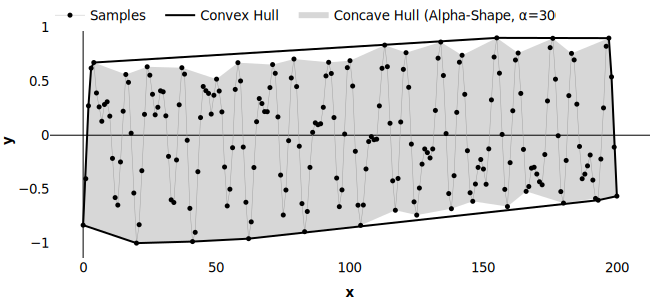
\includegraphics{images/00ConvexHull.pdf}
  \caption{A discrete signal interpreted as a set of points in the Cartesian plane, and the convex and concave hull at $ \alpha=300 $ defined by it.}
  \label{fig:Hulls}
\end{figure}

The alpha shapes approach is used in areas such as detection of features in images \cite{2016VarytimidisAlpha}, reconstruction of surfaces from a cloud of points \cite{2015WuAutomated} and spectroscopy \cite{2019XuModeling}. 

This last work, which involves the estimation and removal of the Blaze function (a kind of envelope) of an echelle spectrograph, being particularly illustrative of the potential synergy between geometric and DSP approaches.

Other steps in the direction of translating geometric algorithms to the context of envelope detection were made by \cite{2015YangSkeleton} via an algorithm based on the construction of a skeleton underlying the digital wave of interest, and also via the direct translation of computer vision methods to the task of envelope detection \cite{2015YangRepresenting}.

Following this path, we present a general approach to envelope detection, exploiting the intrinsic characteristics of a spectrally complex wave, in order to completely avoid the need for manual intervention or parameter tuning.

We start with a brief background of envelope detection in Section \ref{sec:envelope} and define, as specifically as possible, what constitutes a temporal envelope. 

In Section \ref{sec:representation} we explore some simplifications to the task of detecting the envelope of a signal that arise from the envelope definition adopted in this work and simplify the task of envelope detection. 

Section \ref{sec:mapping} explores the geometric characteristics of envelope detection and formalizes how this classic DSP problem can be translated to the geometric problem of finding the shape of a set of points.

We next explore, in Section \ref{sec:curvature}, the concept of discrete curvature, that will be used in Section \ref{sec:envelopedetection}, where the envelope detection algorithm is presented.

Section \ref{sec:quality} discusses the difficulties in the assessment of the quality of an envelope, proposing qualitative and quantitative approaches, and demonstrates that the method propose conforms to four requirements for a physically plausible envelope proposed in \cite{1996Loughlinamplitude}.

In Section \ref{sec:comparison} we compare the presented algorithm with traditional envelope detection methods, both in terms of accuracy and time and present, in Section \ref{sec:extensions},  potential applications of the algorithm, some of which might not be immediately obvious.

% TODO %%%%%%%%%%%%%%%%%%%%%%%%%%%%%%%%%%%%%%
Interactive visualizations are available from the repository prepared for this work \cite{2020TarjanoEnvelope}, that also contains an implementation of the method in pure Python.
A Python module available at the Python Package Index (PyPI) installable via the command `pip install signal-envelope` for convenience, is also available. Besides, those working under Windows 64-bit can benefit from a specialized dynamic library coded in C++ that is automatically used within this module, and can be separately obtained via the release section in the repository.
%%%%%%%%%%%%%%%%%%%%%%%%%%%%%%%%%%%%%%%%%%%%%


\section{Temporal envelope}\label{sec:envelope}

The interest in the theory of envelope detection arose in the analog domain, with the widespread adoption of radio communications, where the problem is typically restricted to artificial waves, often with well-defined frequencies \cite{2011TurnerDemodulation}.

While there is no general formal definition of the envelope of broadband signals \cite{2014Yangnovel,2015Yangtheoretical,2019Jiaempirical}, the general intuition is that an envelope is a smooth curve situated as close as possible to the signal \cite{2019Jiaempirical}.

In this context, the most mathematically sound definition of an envelope involves the representation of its underlying wave as an analytic signal, as introduced by Gabor in 1946 \cite{2007HahnHistory}. In his work, \cite{1946GaborTheory} applies the then relatively new mathematical machinery of the quantum mechanics to unify the time and frequency-domain representations of a wave, showing how the Hilbert transform could be applied to a real signal in order to obtain an equivalent complex signal, later known as the analytic signal.

This analytic signal has the form $ A(t) = S(t) + \mathbb{H}(S(t)) \ \text{i} $ \cite{2016HePraat} where $ S(t) $ is the original real signal. $ \mathbb{H}(S(t)) $, the Hilbert transform of the original signal, becomes the imaginary part of the analytic signal; the envelope of a signal thus represented can be straightforwardly obtained by the computation of the complex modulus of $ \mathbb{H}(S(t)) $.

Despite its widespread use, and effectiveness in the context of narrowband signals, envelope detection techniques based on the Hilbert transform don't behave well for broadband signals \cite{2012DauSpeech, 2019Jiaempirical}, being even physically paradoxical in some cases \cite{1996Loughlinamplitude, 2014Yangnovel}.

Fig. \ref{fig:AnalyticSignal} exemplifies the Hilbert envelope, for a pure sinusoid modulated by a polynomial, illustrating the difference in the smoothness of the envelope in the presence and absence of Gaussian white noise. It is readily noticeable from the Fig. \ref{fig:AnalyticSignal} that, as soon as noise is introduced in the original signal, it is directly reflected in the envelope.

\begin{figure}[ht!]
  \centering
    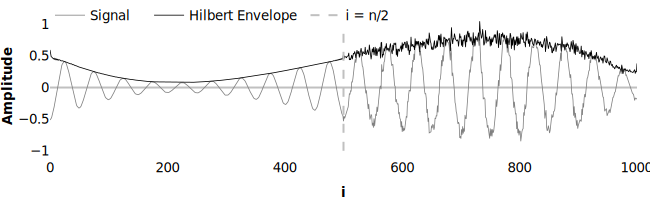
\includegraphics{images/01AnalyticSignal.pdf}
  \caption{Envelope of a pure sinusoid with a local frequency of 20 cycles modulated by a polynomial of degree 3, as obtained by the Hilbert Transform approach. In the first half, the sinusoid is free of noise, while in the second half Gaussian noise with a standard deviation of $ 1/10 $ of the maximum amplitude of the wave was added to the base signal.}
  \label{fig:AnalyticSignal}
\end{figure}

For a real world signal, such as an alto singer sustaining a steady note as shown in Fig. \ref{fig:AnalyticSignalAlto} the Hilbert transform alone provides a poor envelope, since it retains most of the frequencies of the underlying wave. With further processing, however, such as filtering, a smoother output can be obtained.

\begin{figure}[ht!]
  \centering
    \includegraphics{images/01AnalyticSignalAlto.pdf}
  \caption{Representation of an alto singer sustaining a steady note and a comparison of the envelopes obtained by the Hilbert transform with and without further filtering.}
  \label{fig:AnalyticSignalAlto}
\end{figure}

In general, the problem of envelope detection, or demodulation, can be interpreted as the task of, given a continuous wave $ W(t) $, decomposing it in two components $ E(t) $ and $ C(t) $, such that $ W(t) = E(t) C(t) $ \cite{2011TurnerDemodulation}. 

$ E(t) $ represents the slow varying part of the wave, also known as the (temporal) envelope, modulator component, or amplitude modulation (AM) of $ W(t) $, while $ C(t) $ models its fast varying part, called throughout the literature as its (temporal) fine structure, carrier wave, or frequency modulation (FM).

In the case of broadband signals, the problem of envelope detection of an arbitrary wave is ill-posed, in the sense that an infinite number of pairs of $ E(t) $ and $ C(t) $ can result in the same $ W(t) $ \cite{2011TurnerDemodulation, 2013Mengempirical, 1996Loughlinamplitude}.

We address this problem by assuming $ C(t) $ normalized between $ \{-1, 1\}$ or, in other words $ |\max(C(t))| = 1 $. This assumption doesn't cause any loss of generality since, given an arbitrary $ C(t) $, we can obtain its normalization by dividing the function by its absolute global maximum, that is, $ \hat{C}(t) = C(t) / \max(|C(t)|) $, provided that $ \max(|C(t)|) \ne 0 $.

In this work we are concerned with the discrete version of this problem: given a finite digital wave represented by the vector $ \mathbf{w} \in \mathbb{R}^n $, instead of the continuous function $ W(t) $, obtaining the temporal envelope $ \mathbf{e} $ of $ \mathbf{w} $. 

The preceding definitions can be translated to this discrete scenario assuming that the discrete quantities arise from observing the continuous ones at regular time intervals. In that case, the equality $ i = t \ \text{fps} $ can be used to link both settings, where $ i $ is the index of each sample of the digital signal, $ t $ stands for the time in seconds, and fps is the frame rate, or the number of observations made in one second. We can thus define:

\begin{align} \label{eq:Envelope}
\begin{split}
  \text{Given:}& \\
  \mathbf{w} & \in \mathbb{R}^n, \\
  \mathbf{w} & = (w_0, w_1, \cdots, w_{n-1}) \\
  \text{We define:}& \\
  \mathbf{e}, \mathbf{c} & \in \mathbb{R}^n \\
  \mathbf{e} & = (e_0, e_1, \cdots, e_{n-1}), w_i \ge 0 \ \forall \ i, \ 0 \le i \le n-1 \\  
  \mathbf{c} & = (c_0, c_1, \cdots, c_{n-1}), |c_i| \le 1 \ \forall \ i, \ 0 \le i \le n-1 \\
  \mathbf{w} & = \mathbf{e} \odot \mathbf{c} \ \therefore \ w_i = e_i c_i \ \forall \ i, \ 0 \le i \le n-1
\end{split}
\end{align}

The $ \odot $ operator in \ref{eq:Envelope} stands for the Hadamard product, denoting element-wise multiplication of two vectors. Fig. \ref{fig:Envelope} provides an example of the vectors just defined: \textbf{w} is obtained by multiplying the normalized carrier wave \textbf{c} using the envelope \textbf{e}.

\begin{figure}[ht!]
  \centering
    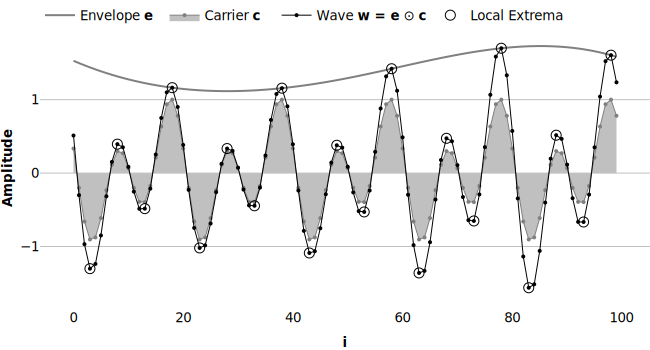
\includegraphics{images/02Envelope.pdf}
  \caption{Example of a discrete wave \textbf{w} composed by the element-wise multiplication of a previously known envelope \textbf{e} and carrier \textbf{c}. The local extrema of \textbf{w} are highlighted with a circle.}
  \label{fig:Envelope}
\end{figure}

In Fig. \ref{fig:Envelope} a signal arising from the multiplication of a known carrier wave \textbf{c} and a known envelope \textbf{e} is shown; this helps to illustrate a key concept: note from Fig. \ref{fig:Envelope} that, only at some local extrema, the envelope can be inferred without prior knowledge of the underlying carrier, being in fact equal to the value of the wave $ w_i $. $ c_i = 1 $ at those points, rendering $ e_i = 1 w_i $.

This realization that the envelope of a wave is defined only at some of the wave's local extrema is crucial, as we can use it to generate a simplified representation of a signal that will make the algorithm more efficient by considering only the local extrema of a given signal.

\section{Simplified Representation} \label{sec:representation}

We start with the definition of a pulse: each time the value of $ w_i$ changes sign, that is, every time the amplitude of the discrete wave \textbf{w} crosses the horizontal axis, the beginning of a pulse is defined, with the next crossing defining its end. This definition is in line with the one presented in \cite{national1996telecommunications}, where a pulse is defined as a rapid change in the amplitude of a signal, followed by a fast return to the baseline value; zero, in our case.

From \ref{fig:Envelope} and the discussion in Section \ref{sec:envelope}, we can see that only the maximum point of a positive pulse or the minimum point of a negative pulse can potentially be equal to the envelope and are, thus, our only points of interest. We can then proceed, for the rest of the method, considering only those points, to great computational economy.

For this reason we define P as the set of the points $ \{P_0, P_1, \cdots, P_{m-1}\} $ where $ P_j = (i_j, \lvert w_{i_j} \lvert) $, that is, $ \lvert w_{i_j} \lvert $, the absolute value of the extrema of each pulse, becomes the ordinate of each point and $ i_j $, its original index, becomes the abscissa.

This relation is illustrated in Fig. \ref{fig:Pulses}. We call it P to emphasize the connection with the pulses of \textbf{w}.
While the exact relation between $ n $, the size of the original signal, and $ m $, the size of the set of points, is dependent on factors such as the frequency and sampling rate of the original wave, the inequality $ m \le n $ holds for all discrete signals. In practice, $ m \ll n $ for most real world signals.

\begin{figure}[ht!]
  \centering
    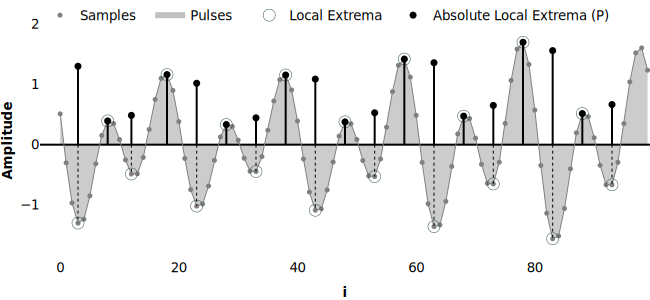
\includegraphics{images/03Pulses.pdf}
  \caption{Example of a discrete wave \textbf{w} divided into pulses, of which the extrema are highlighted with a circle. P is the set of the points $ P_j = (i_j, \lvert w_{i_j} \lvert) $ representing the absolute value of those extrema.}
  \label{fig:Pulses}
\end{figure}


\section{Mapping to the Cartesian coordinate system} \label{sec:mapping}

The points in P are not fit for geometric interpretation yet, since the abscissa and ordinate of their orthogonal coordinate system have different units: in the vertical axis, we have a unit related to the instantaneous amplitude of the wave, while in the horizontal axis we have the index at which each extremum occurs, ultimately a time-related unit. 

Geometrically, we can think of these points as points in a vector space on a non-standard, orthogonal basis vector $ \mathbf{b} = \{ \mathbf{b}_x, \mathbf{b}_y \}$ with $ \mathbf{b}_x = (a, 0), \mathbf{b}_y = (0, i) $ where $ a $ is an amplitude unit such as decibel, a measure of the instantaneous sound pressure, volt or even a fraction of a fixed maximum value. $ i $ represents the index of the sample, and is linked to time by the aforementioned relation $ i = t \ \text{fps} $.

We are interested in representing the point in the standard basis $ \mathbf{s} = \{ \mathbf{s}_x, \mathbf{s}_y \} = \{ (1,0),(0,1) \}$ of this vector space, making the geometric representation consistent.

To achieve that, we divide the ordinate of each point by the average of all ordinates, effectively cancelling the unit of the vertical components of the points. If we proceeded similarly in relation to the horizontal components, 
the direct link between P and \textbf{w} that arises from the fact that the abscissas of the points in P are numerically equivalent to the indices $ i $ of \textbf{w} would be lost.

It is best to leave the abscissas intact and multiply the now unitless vertical coordinates of each point by the average of the difference between the abscissa of a point and the abscissa of the immediately posterior. In this way, we can consider both axes as having unit $ i $, and the relationship is preserved, making it easier to recover the envelope points in the original basis later.

Considering $P_{\mathbf{b}}$ as a point of the set P represented on the original basis and $P_{\mathbf{s}}$ the same point as represented on the standard basis, we can formalize this transformation as in \ref{eq:Basis}:

\begin{align}\label{eq:Basis}
\begin{split}
P_{\mathbf{b}} &= (x_1, x_2) \\
\beta &= \frac{\left( \frac{i_{m-1} - i_m}{m-1} \right)}{\left( \frac{\sum_{j=0}^{m-1} \lvert w_j \lvert}{m} \right)}  \\
P_{\mathbf{s}} &= (x_1, \beta x_2) \quad \forall \  P \in \text{P} \\ 
\end{split}
\end{align}

The effect of this normalization can be seen in the points shown in Fig. \ref{fig:Coordinates}, shown in scale for both basis. We can consider our points now residing in the Cartesian coordinate system.

\begin{figure}[ht!]
  \centering
    \includegraphics{images/04Coordinates.pdf}
  \caption{The set of points P, in both the original (top) and standard (bottom) coordinate basis, shown in scale.}
  \label{fig:Coordinates}
\end{figure}


\section{Discrete Curvature Estimation} \label{sec:curvature}

Having established a transformation from the original space of the two-dimensional representation of a discrete wave to the Cartesian coordinate system and, thus, a way to consistently transform our simplified description of a discrete signal into a set of points in the plane, the shape of which can be estimated with the use of geometric algorithms.

The goal of those algorithms, such as the convex hull and the alpha-shapes, is to discriminate which points of a set are part of its frontier.

A formal definition of alpha-shapes is given at \cite{1983Edelsbrunnershape}. In the context of this work, gaining the intuition of the algorithm is more important, and thus the explanation of the alpha-shapes algorithm presented in \cite{1994EdelsbrunnerThree} can be more insightful.

The explanation, translated to our context, invites one to think of the plane were the samples are represented as a soft material, such as Styrofoam. The samples themselves are a harder material, such as rock, and occupy a fixed position in this plane. The alpha shapes algorithm consists of carving this plane from the outside of those points, with a circular eraser of fixed radius $ \alpha $. In the end of the process, the remaining Styrofoam that couldn't be erased due to the impeding rocks is the alpha-shape of this set of points.

Alternatively, one can picture a circle of fixed radius being rolled above the signal, and marking the points it touches as envelope points.

To employ an alpha shapes inspired algorithm in this set of points, however, the radius $ r $ of such circle must be estimated, and for that a measure of discrete curvature is needed.

Discrete curvature estimation is an important task in image processing \cite{2010FleischmannNovel} for which no default definition exists. 

The two general approaches are the derivation of direct methods that use characteristics of the discrete curve to calculate the curvature, or the use of the curvature of a smooth, continuous curve fitted to the original discrete curve \cite{2001CoeurjollyDiscrete}.

Concerning direct methods \cite{2014CarrollSurvey}, for example, derive three such definitions based on the approximation of a circle by an inscribed, centered and circumscribed polygon. In the context of three-dimensional meshes, \cite{2016VasaMultivariate} evaluate a range of existing estimators from a multivariate point of view.

Those approaches define the discrete curvature in relation to the vertices of a discrete curve (or mesh, in the three-dimensional case). Instead, we are interested in the change of direction, what the term curvature ultimately means, between two adjacent points.

Since we are dealing with a potentially large set of points, it is important for this measure to act locally, to assure $ O(n) $ complexity.

Thus, the set V of the vectors from each point of P to the next, shown in the Fig. \ref{fig:Vectors}, will be used to estimate the average curvature of P: We will calculate the equivalent circle for each vector, and average the values thus obtained to infer the average curvature of the whole discrete curve. 

\begin{figure}[ht!]
  \centering
    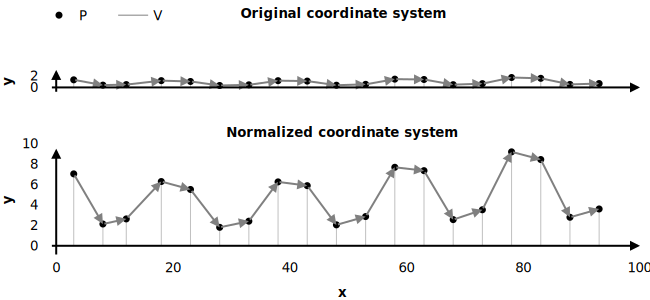
\includegraphics{images/04Vectors.pdf}
  \caption{The set of points P and the set V of vectors between two adjacent points of P, in the normalized coordinate system.}
  \label{fig:Vectors}
\end{figure}

We formalize the set of vectors V in Eq. \ref{eq:Vectors} below.

\begin{align} \label{eq:Vectors}
\text{V} = \{ v_0, v_1, \cdots, v_{m-2} \} \quad \text{where} \quad v_k = P_{j+1} - P_j \quad \forall \quad 0 \le k \le m-2
\end{align}


\subsection{The Equivalent Circle Approach} 

We thus proceed to define a discrete curvature measure over the edges of a discrete curve. To that end we are going to apply the definition of smooth curvature as the rate of change of the unit tangent to a curve. This definition is convenient, since it is equivalent to that of the osculating circle \cite{2016VasaMesh}, the value we are interested in finding.

One of those edges, in the form of the vector $ v_k \in \text{V} $, is singled out in Fig. \ref{fig:DiscreteCurvature}. $ v_k $ represents the net displacement of the envelope from the extrema $ P_{j} = (x_j, y_j) $ to $ P_{j+1} = (x_{j+1}, y_{j+1}) $. Since we don't yet know which points of P are part of the envelope, instead of assuming that the trajectory before $ P_{j} $ passes through $ P_{j-1} $, it is more prudent to assume that it can have passed anywhere in the line segment from points $ (x_j - (x_{j+1} - x_j), y_j - (y_{j+1} - y_j)) $ to $ (x_j - (x_{j+1} - x_j), y_j + (y_{j+1} - y_j)) $, the bold line segment before $ v_k $ in Fig. \ref{fig:DiscreteCurvature}.

That is because all we can safely assume from $ v_k $ is that, in the immediate vicinity of the vector, the envelope is capable of a vertical displacement of $ v_{k,y} $ in the same time as it performs a horizontal displacement of $ v_{k,x} $;

Since this is true for all the vectors $ v_k \in \text{V} $, we can consider that, on average, the envelope insides horizontally at $ P_{j} $.

The rationale then is to find, for each vector $ v_k $, the radius $ r_k $ of the equivalent circle whose tangent has the same change in direction, in the same horizontal distance, as the vector, as shown in Fig. \ref{fig:DiscreteCurvature}. The average curvature of P will then be obtained by the average of all radii $ r_k $.

From Fig. \ref{fig:DiscreteCurvature} one can see that $ r_k = v_{k,x} / \sin(\theta_k) $ where $ v_{k,x} $ is the component of $ v_k $ in the horizontal direction; $ \theta_k $ itself can be obtained using the slope $ m_0 = 0 $ of the horizontal line and the slope $ m_k = v_{k,y} / v_{k,x} $ defined by $ v_k $ using the equality $ \theta_k = \arctan \big( (m_k - m_0) / (1 + m_k m_0) \big) $.

\begin{figure}[ht!]
  \centering
    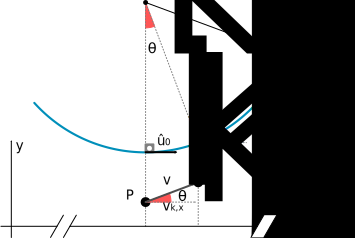
\includegraphics{images/05DiscreteCurvature.pdf}
  \caption{The tangent unit vector of the circle changes from the horizontal direction in $ \hat{u}_0 $ to an inclination of $ \theta_k $ in $ \hat{u}_1 $, $ \theta_k $ being the angle that the vector $ v_k $ makes with the horizontal direction.}
  \label{fig:DiscreteCurvature}
\end{figure}

The radius $ r_k $ of the circle equivalent to each $ v_k $ is defined in Eq. \ref{eq:Radius}. This equation has the desirable property that $ v_{k,y} \to 0 \implies v_{k,y} \to \infty $, that is, the radius tends to infinity when no vertical oscillation occurs, effectively turning the circle into a line. 

The radius is also directly proportional to $ v_{k,x} $, making the radius larger the more the points are horizontally far from each other.

\begin{align} \label{eq:Radius}
  r_k = \frac{v_{k,x} \sqrt{v_{k,x}^2 + v_{k,y}^2}}{ v_{k,y}}
\end{align}

For calculation purposes, however, this can pose a problem, as a zero could make its way into the denominator of a fraction; in the actual algorithm, the quantity calculated for each vector is the curvature itself, that is, the inverse of each radius $ r_k $. In this way, the problem is avoided, since $ v_{k,x} $ is guaranteed to be greater than zero. The average of curvatures is then inverted in order to obtain the average radius $ \overline{r} $, as illustrated in Eq. \ref{eq:Curvature}.

\begin{align} \label{eq:Curvature}
\overline{r} = \left( \frac{\sum\limits_{k=0}^{m-2} \left( \frac{ v_{k,y}}{v_{k,x} \sqrt{v_{k,x}^2 + v_{k,y}^2}} \right)}{m-2} \right)^{-1}
\end{align}

\section{Identifying the envelope} \label{sec:envelopedetection}

We need now to construct an algorithm, using the radius just obtained, to identify the points that belong to the envelope. Generally, alpha-shapes based algorithms resort to the construction of the Delaunay triangulation of the set of points, that is latter filtered to contain only the outer edges. We can adopt a more straightforward method, as our points have a sequential structure. 

It is worth noting that, although that is the case throughout this work, the original signal doesn't need to be sampled at equal intervals.

Let $ x_o, y_o \in \mathbb{R}, \quad 0 \le y_o < +\infty $ be the coordinates of the center of a circle with radius $ r $, that can be placed anywhere in the upper plane of the coordinate system;

Let $ P_a, P_b, P_c \in \text{P}, \quad P_a \ne P_b \ne P_c $ be three different points of the set P;

For all circles of center $ x_o, y_o $ and radius $ r $ that can be constructed to pass through any two different points of P, that is, $ \forall \quad P_b, P_c $ such that $ (P_{b,x} - x_o)^2 + (P_{b,y} - y_o)^2 = (P_{c,x} - x_o)^2 + (P_{c,y} - y_o)^2 = r^2 $, $ P_a $ will be part of the set $ E $ of the points belonging to the envelope if and only if none of those circles contain $ P_a $, or $ P_a \in \text{E} \leftrightarrow (P_{b,x} - x_o)^2 + (P_{b,y} - y_o)^2 > r^2 $. Summarizing this, we have Eq. \ref{eq:InEnvelope}:

\begin{align} \label{eq:InEnvelope}
\begin{split}
& P_a \in \text{E} \leftrightarrow (P_{b,x} - x_o)^2 + (P_{b,y} - y_o)^2 > r^2, \\
& \forall \ P_b, P_c \mid (P_{b,x} - x_o)^2 + (P_{b,y} - y_o)^2 = (P_{c,x} - x_o)^2 + (P_{c,y} - y_o)^2 = r^2, \\
& P_a, P_b, P_c \in \text{P}, \quad P_a \ne P_b \ne P_c \quad \text{and} \quad x_o, y_o \in \mathbb{R}, \quad 0 \le y_o < +\infty
\end{split}
\end{align}

The algorithm follows directly from the definition in \ref{eq:InEnvelope} after noting that the first and last members of P will always be part of the envelope, since they are reachable by a circle of any radius $ r $. From $ P_0 $, our first pivot point, we construct circles passing through $ P_1, P_2, \cdots, P_d $ until a circle that doesn't contain any point in P is found; $ P_d $ then becomes the new pivot point and is included in E, and this process continues until $ P_{m-1} $ is reached.

The procedure is formalized in the algorithm \ref{FindEnvelope}. We don't provide similar algorithmic descriptions of the preceding steps since the Python implementation available at \cite{2020TarjanoEnvelope} can easily serve as pseudocode.

\begin{algorithm}[ht!]
\caption{Retrieve Envelope} \label{FindEnvelope}
\begin{algorithmic}
\STATE \textbf{Given} $ \text{P} = \{P_0, P_1, \cdots, P_{m-1}\}, r $, \textbf{circle}, a function that returns the center of a circle of a given radius passing through two points and \textbf{distance}, a function that returns the Euclidean distance between two points,
\STATE \textbf{Let} $ \text{E} = \{ P_0 \}, \text{id1} = 0, \text{id2} = 1 $
\STATE \textbf{Define} $ P_c = \text{point}, \text{empty} = \text{boolean} $
\WHILE {$ \text{id2} < m $}
  \STATE $ P_c \leftarrow \textbf{circle}(r, P_\text{id1}, P_\text{id2}) $
  \STATE empty $ \leftarrow $ \TRUE 
  \FOR{$ i = \text{id2} + 1 $ \TO $ m $}
    \IF {$ \textbf{distance}(P_c, P_i) < r $}
      \STATE empty $ \leftarrow $ \FALSE
      \STATE id2 $ \leftarrow \text{id2} + 1 $
      \STATE \textbf{break}
    \ENDIF
  \ENDFOR
  \IF {empty}
    \STATE E $ \leftarrow $ E $ \cup \ \{ P_\text{id2} \} $
    \STATE id1 $ \leftarrow $ id2
    \STATE id2 $ \leftarrow \text{id2} + 1 $
  \ENDIF
\ENDWHILE
\end{algorithmic}
\end{algorithm}

The set E obtained via algorithm \ref{FindEnvelope} is a subset of P, and thus also a set of points in the Euclidean space. 

Recall from section \ref{sec:mapping} that the vertical coordinates of these points are currently scaled by the change of basis described in Eq. \ref{eq:Basis}, in relation to the original signal as represented in his original basis. We could invert this transformation, but since we were careful to maintain the direct link between the horizontal coordinates in both basis, we can simply consider the horizontal coordinates of P as the indices of samples of the original discrete signal, whose absolute value are part of the envelope.

The most straightforward way to transform those points into the vector $ \textbf{e} \in \mathbb{R}^n $ is via linear interpolation, the approach used in this work.

It is worth noting, however, that many other procedures are available, both for the interpolation and the smooth approximation of points. Depending on the intended use of the envelope, k-curves interpolation \cite{2017Yank}is a specially interesting approach, since it guarantees that the maximum curvature occurs at the interpolated points.

\section{Quality of an envelope} \label{sec:quality}

The lack of a precise definition of what an envelope is makes the assessment of the quality of an envelope a difficult task, for which there are no agreed-upon objective metrics. Recalling Fig. \ref{fig:Envelope}, however, and the accompanying discussion, if one divides, element-wise, the original signal by the envelope, the carrier wave thus obtained is expected to be bounded between -1 and 1.

Figs. \ref{fig:spokenvoice}, \ref{fig:singer_voice} and \ref{fig:Bend} present discrete waves \textbf{w}, their extracted envelope \textbf{e}, and the inferred carrier \textbf{c}, obtained after dividing, element-wise, the original signal by its extracted.

From Fig. \ref{fig:spokenvoice} it can be seen that the algorithm performs well under the carrier metric. This is especially remarkable for the case of spoken voice, a notorious complex wave with fast changes in pitch and high noise content.

\begin{figure}[ht!]
  \centering
    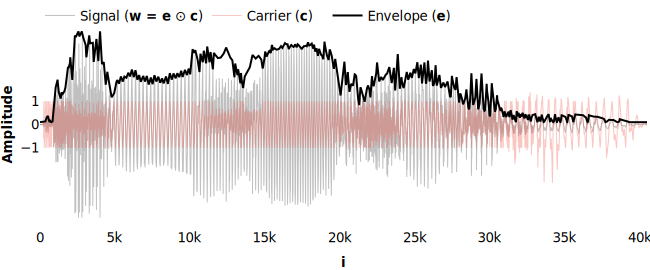
\includegraphics{images/06Graph_spoken_voice.pdf}
  \caption{Signal, envelope and carrier for a record of male voice uttering the word “amazing”.}
  \label{fig:spokenvoice}
\end{figure}

Those characteristics are in stark contrast with those of the sang voice in Fig. \ref{fig:singer_voice}, where a recording of an alto singer sustaining a steady note is shown; there, the wave is almost periodic, with a stable waveform and envelope.

\begin{figure}[ht!]
  \centering
    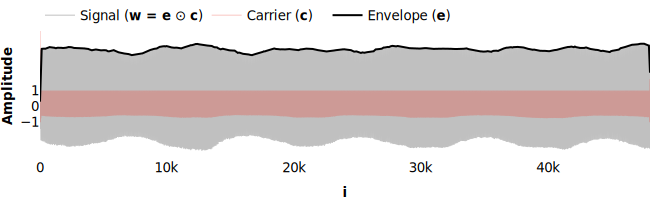
\includegraphics{images/06Graph_alto.pdf}
  \caption{Signal, envelope and carrier for a record of an alto singer.}
  \label{fig:singer_voice}
\end{figure}

Fig. \ref{fig:Bend} shows the envelope in the case of a bend performed in an electric guitar. The variations in frequency in the signal didn't affect the envelope extracted.

\begin{figure}[ht!]
  \centering
    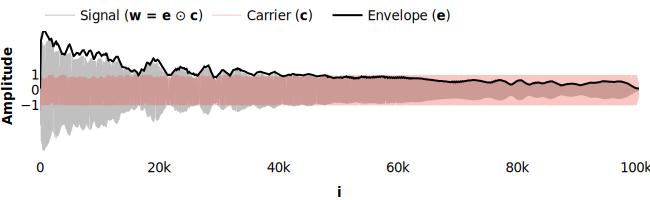
\includegraphics{images/06Graph_bend.pdf}
  \caption{Signal, envelope and carrier for a record of a bend performed on an electric guitar.}
  \label{fig:Bend}
\end{figure}

\subsection{Theoretical guarantees}

In an effort to formalize the assessment of the quality of amplitude and frequency modulations of a signal, \cite{1996Loughlinamplitude} proposed some theoretical conditions necessary, but not sufficient, to ensure the physical plausibility of an envelope. 

We comment below on how those conditions translate to the discrete setting, and show that the algorithm here presented satisfies the four conditions presented.

The first one states that, if a signal is bounded in magnitude, then its envelope should be, as well. Our algorithm complies with this requirement, as the envelope is composed of selected samples from the original signal itself.

More formally, we have the set P of the absolute values of the local extrema of the original signal $ \mathbf{w} = (w_0, w_1, \cdots, w_{n-1}) $ that contains, by definition, the global extrema of $ \mathbf{w} $.
The set E of the points that belong to the envelope is a subset of P. We can thus write Eq. \ref{eq:Req1}:

\begin{align} \label{eq:Req1}
\begin{split}
\text{P} &= \{ P_0, P_1, \cdots, P_{m-1} \} \quad \text{where} \quad P_j = (i_j, \lvert w_{i_j} \lvert) \quad \forall \quad 0 \le j \le m-1 \\
\text{E} &\subset \text{P} \implies \max (\text{E}) \le \max (\text{P}) = \max (|w_0|, |w_1|, \cdots, |w_{n-1}|)
\end{split}
\end{align}

If the amplitude of the original signal is bounded, that is $ \max (|w_0|, |w_1|, \cdots, |w_{n-1}|) = b \in \mathbb{R} $, not only the amplitude of the envelope is bounded, as required, but is guaranteed to have the same bound $ b $.

The second statement dictates that if the signal has a finite frequency range, that frequency range must not be exceeded by the carrier wave. 

To see that this condition holds for the proposed method, consider a discrete signal $ \mathbf{w} = (w_0, w_1, \cdots, w_{n-1}) $, where all the absolute values of its local extrema are greater than one.

This requirement doesn't imply loss of generality since, for an arbitrary signal, we can assure this condition by dividing all samples by the value of the minimum absolute local extrema. 

The relation $ \min(\text{E}) \ge 1 $ thus holds, since $ \text{E} \subset \text{P}$. 

Provided that one uses a method that preserves the original bounds when interpolating the points in E, such as linear interpolation, we can be sure that all the points in the envelope vector $ \mathbf{e} = (e_0, e_1, \cdots, e_{n-1}) $ are also greater than one.

Recalling Eq. \ref{eq:Envelope}, where the relation between the original signal, the carrier and the envelope was defined as $ \mathbf{w} = \mathbf{e} \odot \mathbf{c} $, we can write the magnitude of an arbitrary frequency of the original signal ($ m_\mathbf{w}(f) $) and, likewise, the magnitude of an arbitrary frequency of the carrier ($ m_\mathbf{c}(f) $) in terms of the Discrete Fourier Transform (DFT) as in Eq. \ref{eq:DFT}:

\begin{align} \label{eq:DFT}
\begin{split}
m_\mathbf{w}(f) &= \sum_{k=0}^{n-1} \sqrt{\left( w_k \cos(2 \pi k f / n) \right)^2 + \left( w_k \sin(2 \pi k f / n) \right)^2} \\
m_\mathbf{c}(f) &= \sum_{k=0}^{n-1} \sqrt{\left( \frac{w_k}{e_k} \cos(2 \pi k f / n) \right)^2 + \left( \frac{w_k}{e_k} \sin(2 \pi k f / n) \right)^2} 
\end{split}
\end{align}

For any given frequency $ f $, both $ m_\mathbf{w}(f) $ and $ m_\mathbf{c}(f) $ are nonnegative. Also, since $ e_k \ge 1 \ \forall \ k, 0 \le k \le n - 1 $ we establish that $ 0 \le m_\mathbf{c}(f) \le m_\mathbf{w}(f) \ \forall \ f $ which is a more restrictive condition than the original: If $ \mathbf{w} $ has a finite frequency range, the magnitude of frequencies outside that range are zero, as are those of the same frequencies of the carrier $ \mathbf{c} $.


The third condition states that a physically plausible algorithm should, for a signal $ \mathbf{w} $ of constant amplitude $ a > 0, \ a \in \mathbb{R} $ and constant frequency, of the form $ a \cos(\omega i + \phi) $, result in a constant envelope $ \mathbf{e} $ of magnitude $ a $ and o a carrier wave $ \mathbf{c} $ of the form $ \cos(\omega i + \phi) $.

An example of such behaviour can be observed in Fig. \ref{fig:Comparison_sinusoid}, where the envelope of a simple sinusoid is shown. To see that this is always the case, note that all the extrema of a sinusoid are of the form $ a (\pm 1) $ and $ P_j = (i_j, \lvert a (\pm 1) \lvert) = (i_j, a) \ \forall P_j \in \text{P} $. As $ \text{E} \subset \text{P} $, we have that the envelope $ \mathbf{e} = (a, a, \cdots, a) $ and is, thus constant. Likewise, since $ \mathbf{w} = \mathbf{e} \odot \mathbf{c} $, we have $ c_i = a \cos(\omega i + \phi) / a = \cos(\omega i + \phi) \ \forall \ i, 0 \le i \le n - 1 $.

The fourth and last condition states that if a wave is multiplied by a constant, its envelope should also be multiplied by the same constant. 

Recall from section \ref{sec:mapping} that, before the extraction of the envelope, the original points undergo a change of basis to lie in the Cartesian coordinate system. After the extraction, the inverse operation is performed on the points of the Envelope.

Consider a discrete signal $ \mathbf{w} = (w_0, w_1, \cdots, w_{n-1}) $ and the set P of its absolute extrema, represented in the standard basis, $ \text{P} = \{ P_0, P_1, \cdots, P_{m-1} \}, \quad P_j = (i_j, \beta \lvert w_{i_j} \lvert) $, where $ \beta $ is obtained from Eq. \ref{eq:Basis}.

Given a constant $ \alpha > 0, \alpha \in \mathbb{R} $, we can define the scaled signal as $ \mathbf{w}^\prime = (\alpha w_0, \alpha w_1, \cdots, \alpha w_{n-1}) $. Observing, from Eq. \ref{eq:Basis}, that $ \alpha $ can be factored out of denominator of the summation, we have $ \beta^\prime = \beta / \alpha $ and the new set $ \text{P}^\prime = \{ P^\prime_0, P^\prime_1, \cdots, P^\prime_{m-1} \}, \quad P^\prime_j = (i_j, \frac{\beta}{\alpha} \lvert \alpha w_{i_j} \lvert) $ is equal to the set P for the signal before scaling.

This guarantees that the same subset of points E will be identified as part of the envelope in both cases.
In the respective original basis system, applying the inverse change of basis, those points are $ P_j = (i_j, \frac{\beta}{\beta} \lvert w_{i_j} \lvert)  \quad \forall \  P \in \text{E} $, for the original signal, and $ P^\prime_j = (i_j, \frac{\alpha}{\beta}\frac{\beta}{\alpha} \lvert \alpha w_{i_j} \lvert) $ for the scaled signal.

\subsection{Reference envelope}

In order to obtain a numeric indicator of the quality of an envelope, we construct a reference envelope, that trades off practical applicability in favour of mathematical formality.
In \cite{1992BruceCurves} the envelope is defined as the boundary of the region filled by a family of curves. Fig. \ref{fig:RefEnvelopeTheory} illustrates this concept, for a family of sinusoids that share the same frequency and amplitude, and whose phases vary from 0 to $ 2 \pi $.

\begin{figure}[ht!]
  \centering
    \includegraphics{images/09RefEnvelopeTheory.pdf}
  \caption{Envelope as the boundary of the region filled by a family of curves, for a family of sinusoids with the same frequency and amplitude, modulated by a polynomial.}
  \label{fig:RefEnvelopeTheory}
\end{figure}

In practical applications, one seldom has access to a family of curves, instead being interested in obtaining the envelope of a single signal. Nevertheless, an approximation can be obtained, by shifting the original signal along its initial position in the horizontal axis, in order to cover the time of one period of the signal.
Fig. \ref{fig:RefEnvelope} shows the reference envelope for the sound of a tom.

\begin{figure}[ht!]
  \centering
    \includegraphics{images/10RefEnvelope.pdf}
  \caption{Reference envelope obtained by shifting the original signal, for part of a sample of a tom.}
  \label{fig:RefEnvelope}
\end{figure}

Since envelope is not smooth, being composed of a series of horizontal segments, as can be seen in \ref{fig:RefEnvelope}, besides being computationally expensive to calculate. However, arising from a mathematically sound base, it can serve as a reference to infer the quality of more empirical methods.


\subsection{Comparison with traditional algorithms}\label{sec:comparison}

Direct comparison with many of the more recent algorithms is made difficult by the unavailability of digital implementations of such works, many designed to process analog signals \cite[e.g.,][]{2018AssefModeling}.

Nevertheless, insight can be gained from a comparison of the results of the method here proposed with some of the most common envelope extraction algorithms. Specifically, we compare the present method with the following approaches:

\begin{enumerate}
\item Smoothing: This is a relatively simple procedure that, applied to the absolute values of a discrete signal, can provide an approximation of the variation of its amplitude in time. We use the Savitzky-Golay algorithm \cite{1964SavitzkySmoothing} with a window width of 3001 samples and a cubic polynomial.
\item Filtering: The absolute value of the wave is filtered using a digital implementation of the Butterworth \cite{butterworth1930theory} low pass filter. We use an order 2 filter with a cut-off frequency of 10 Hz.
\item Hilbert Transform: We apply the Hilbert transform to the original signal, filtering the absolute value of the complex result with a Butterworth filter with a cut-off frequency of 1/10 of the fundamental frequency of the original signal.
\end{enumerate}

In Fig. \ref{fig:Comparison_sinusoid} we illustrate the envelope extracted by the conventional algorithms, contrasting it with the result of the method presented in this work, for a simple sinusoid. 
Only the present algorithm and the one based on the Hilbert transform comply with the third condition proposed by \cite{1996Loughlinamplitude}, that states that the envelope of a periodic wave should be a straight line.

\begin{figure}[ht!]
  \centering
    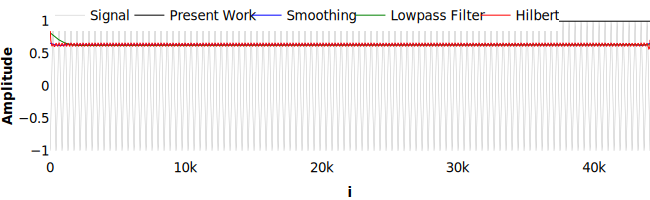
\includegraphics{images/07Comparison_sinusoid.pdf}
  \caption{Comparison of envelope detection algorithms for a simple sinusoid. The envelope for the Hilbert transform and for the present work are coincident in the image.}
  \label{fig:Comparison_sinusoid}
\end{figure}

For a recording of the key 33 of a grand piano, where parts of the sound, specially at the start, are highly percussive and noisy, the Hilbert approach presents a considerable deviation, as can be seen in Fig. \ref{fig:Comparison_piano}.

\begin{figure}[ht!]
  \centering
    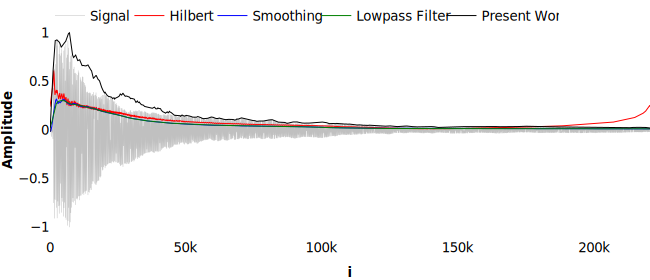
\includegraphics{images/07Comparison_piano.pdf}
  \caption{Comparison of envelope detection algorithms for the recording of the key 33 of a grand piano}
  \label{fig:Comparison_piano}
\end{figure}

In Fig. \ref{fig:Comparison_soprano} all envelopes exhibit a similar movement along the samples, but the ones generated by traditional algorithms are consistently undershooting the original wave.

\begin{figure}[ht!]
  \centering
    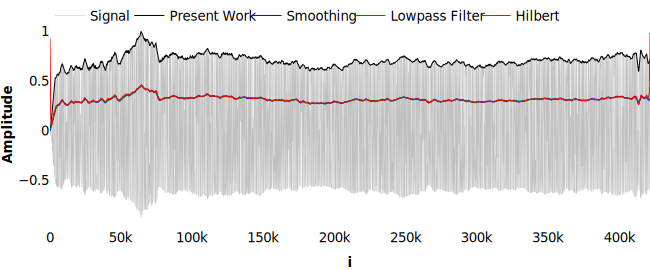
\includegraphics{images/07Comparison_soprano.pdf}
  \caption{Comparison of envelope detection algorithms for the recording of the vocalization of a soprano singer}
  \label{fig:Comparison_soprano}
\end{figure}

Besides, the traditional methods demanded careful choice of parameters. In the case of the Hilbert transform, post-processing in the form of filtering was applied, and an appropriate cut-off frequency had to be chosen. That is in contrast with our method, that organically tunes itself via the automatic choice of the radius of the circle representing the average discrete curvature of the signal.

Table \ref{table:Error_comparison} presents the average of the absolute errors of the techniques, when compared with the reference envelope introduced in the end of section \ref{sec:quality}

\begin{table}[ht!]
\centering
\begin{tabular}{lcccc}
\hline
\multicolumn{5}{c}{\textbf{Average error per frame}} \\
Signal & Present Work & Smoothing & Low pass & Hilbert \\ 
\hline
alto  & 0.001 & 0.337 & 0.342 & 0.163 \\
bend  & 0.000 & 0.029 & 0.030 & 0.008 \\
brass & 0.001 & 0.107 & 0.107 & 0.038 \\
nonperiodic & 0.000 & 0.211 & 0.158 & 0.000 \\
piano & 0.003 & 0.016 & 0.016 & 0.007 \\
sinusoid & 0.000 & 0.132 & 0.131 & 0.000 \\
soprano & 0.000 & 0.155 & 0.155 & 0.044 \\
spoken\_voice & 0.006 & 0.109 & 0.110 & 0.045 \\
tom   & 0.001 & 0.011 & 0.015 & 0.005 \\
\hline
Average & 0.001 & 0.123 & 0.118 & 0.035 \\
frac. of max. & 0.010 & 1.000 & 0.961 & 0.281 \\
\end{tabular}
\caption{Comparison of the average errors of the algorithm presented in this work with the most common methods of digital envelope identification. The discrete waves used were normalized between -1 and 1. The average is between the absolute value of those waves and the envelope divided by two.}
\label{table:Error_comparison}
\end{table}

We can see from the table \ref{table:Error_comparison} that the method presented here consistently outperforms the traditional approaches for all waves tested, yielding an error of less than 2\% on average, of the error of the traditional methods. 

The times taken for the algorithms to process each signal are shown in \ref{table:Time_comparison}. 
The Python source for the tests, as well as the samples used, are available at the repository dedicated to this work, in the file “Comparison of Envelope Algorithms.py”.

The methods were performed as described in the beginning of this section, using the implementations available at the Scipy library, under the Signal processing module. The presented algorithm, is on average, the second-fastest.

\begin{table}[ht!]
\centering
\begin{tabular}{lcccc}
\hline
\multicolumn{5}{c}{\textbf{Time in seconds}} \\
Signal  & Present Work & Smoothing & Low pass & Hilbert \\ 
\hline
alto  & 0.010 & 0.096 & 0.007 & 0.006 \\
bend  & 0.009 & 0.146 & 0.005 & 0.067 \\
brass & 0.015 & 0.253 & 0.005 & 0.035 \\
nonperiodic & 0.002 & 0.064 & 0.003 & 0.007 \\
piano & 0.022 & 0.316 & 0.009 & 0.030 \\
sinusoid & 0.003 & 0.069 & 0.003 & 0.006 \\
soprano & 0.111 & 0.574 & 0.013 & 0.293 \\
spoken\_voice & 0.003 & 0.062 & 0.003 & 0.017 \\
tom   & 0.002 & 0.070 & 0.001 & 0.004 \\
\hline
Average & 0.020 & 0.183 & 0.005 & 0.052 \\
frac. of max. & 0.108 & 1.000 & 0.030 & 0.283 \\
\end{tabular}
\caption{Comparison of the processing time of the algorithm presented in this work with the most common methods of digital envelope detection.}
\label{table:Time_comparison}
\end{table}

\section{Extensions} \label{sec:extensions}

In this section we comment briefly on some characteristics and extensions of the presented algorithm, in order to suggest possible applications beyond envelope extraction. One of the less obvious is, perhaps, its use in the segmentation of a signal into pseudo cycles.

\subsection{Superior and inferior envelopes}

In practice, is not uncommon for a discrete wave, especially in the case of sound, to present somewhat different superior and inferior contours; in those cases, the algorithm can be easily adapted to infer from the positive and negative pulses defined by the original wave to define two independent “envelopes”, that we are going to call superior and inferior frontiers.

If we split P, as defined in section \ref{sec:representation}, into $\text{P}^+$, the set of the local maxima of the original signal and $\text{P}^-$, the set of its local minima, we can apply the remaining steps of the algorithm in those two sets independently, arriving at a positive and a negative frontier.

Fig. \ref{fig:FullFrontiers} illustrates these frontiers for six diverse discrete sound waves, as well as an in-detail view of the highlighted segment for each signal. All waves are records of physical sounds, chosen to represent the applicability of the algorithm in real-world scenarios. The implementation available at the PyPI repository provides an option to extract the frontiers.

\begin{figure}[ht!]
  \centering
    \includegraphics{images/08FullFrontiers.pdf}
  \caption{Positive and negative frontiers of six digital waves, as extracted by the algorithm here presented. For each wave, the region highlighted in black is shown in detail besides the whole wave. For each wave, the horizontal axis is the sample number $ i $, while the vertical axis is the normalized amplitude. All 6 waves were recorded at 44100 fps.}
  \label{fig:FullFrontiers}
\end{figure}

The frontiers were are satisfactorily detected in the case of harmonic and inharmonic sounds, and are robust in relation to the number of samples and the frequencies of the waves. It is worth noting that the positive and negative frontiers are generally smoother than the unified envelope and seems to conform better to the countours of the underlying digital signal.


\subsection{Simplified spectral representation} 

The temporal envelope adds complexity to the spectral representation of a wave \cite{2019TarjanoNeuro}, and an accurate description of the envelope, while describing the evolution of the instantaneous amplitude of a signal in time, would also simplify further spectral analysis. 

Fig. \ref{fig:Fourier} shows the frequency-domain power spectrum for the wave and the carrier presented in \ref{fig:Envelope}. For the carrier, the power spectrum presents two nonzero values, while the power spectrum for the wave composed of the carrier modulated by the envelope is more complex.

\begin{figure}[ht!]
  \centering
    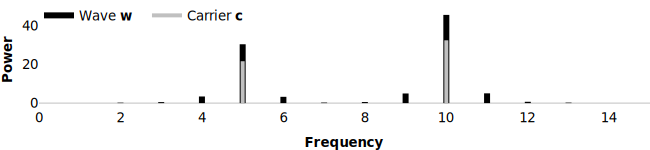
\includegraphics{images/11Fourier.pdf}
  \caption{Fourier power spectrum for the wave and carrier shown in \ref{fig:Envelope}.}
  \label{fig:Fourier}
\end{figure}

Fig. \ref{fig:FourierBend} shows part the power spectra for both the original wave and the carrier obtained by the present algorithm, for the guitar bend sound in Fig. \ref{fig:Bend}, around its fundamental frequency. Two prominent frequencies can be seen, the initial and final notes of the bend. In the carrier, the other frequencies appear more smooth.

\begin{figure}[ht!]
  \centering
    \includegraphics{images/12Fourier.pdf}
  \caption{Fourier power spectrum for the wave and carrier of the sound of a guitar bend shown in Fig. \ref{fig:Bend}.}
  \label{fig:FourierBend}
\end{figure}

\subsection{Approximated location of pseudo-cycles} 

The algorithm developed in this work naturally divides a signal into its pseudo-cycles, pinpointing them in the time-domain, as illustrated in Fig. \ref{fig:singer_voice}, for the sound of an alto singer singing a sustained note, as in Fig. \ref{fig:singer_voice}. 

The vertical lines mark the indices of the samples that belong to the positive frontier of the original signal, and the section between each vertical line isolates a pseudo cycle of the wave. Note that, although two local maxima exist in each pseudo cycle, only the largest was marked.

\begin{figure}[ht!]
  \centering
    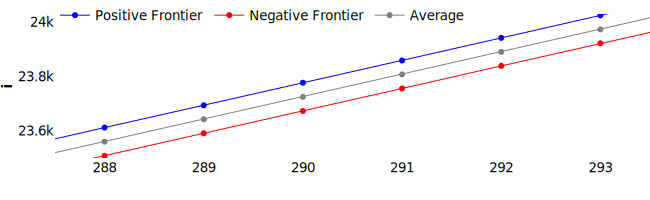
\includegraphics{images/09PCs.pdf}
  \caption{Section of the digital wave illustrated in \ref{fig:singer_voice}, with vertical lines at the indices of the samples that belong to the positive frontier.}
  \label{fig:PCs}
\end{figure}

Therefore, using those indices, one can split a discrete wave into its pseudo cycles. One application of that is illustrated in Fig. \ref{fig:AvgPc}: It shows the superposition of the extracted pseudo cycles, after being normalized by length, and their average. They were also rotated to make their starting point more close to zero.

This same average is shown shifted, to exemplify that approximate $C^0$ and $C^1$ continuity is achieved. This can be seen as the average waveform of the original discrete signal, and can be used, along with the information of its envelope, to generate an alternative representation of the wave, useful, for example, for compression and classification purposes.

\begin{figure}[ht!]
  \centering
    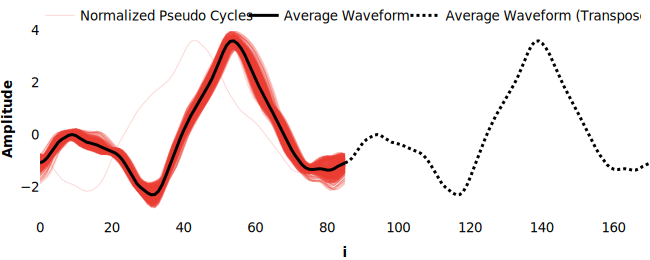
\includegraphics{images/10AvgPc.pdf}
  \caption{Pseudo-cycles of the wave illustrated in \ref{fig:singer_voice}, segmented and superposed, and their average. The average is also shown shifted by one average period, to illustrate the average continuity.}
  \label{fig:AvgPc}
\end{figure}


\section{Conclusion}
This work fills a gap identified in the theory of digital signal processing, where the lack of general procedures for the accurate identification of the temporal envelope of arbitrary waves poses an obstacle to the complete description and eventual manipulation of signals.

By presenting a general approach for envelope detection, and eliminating the need for parameter tuning, we expect to facilitate further research in the many areas that rely on envelope detection techniques, and improve already existing algorithms that have envelope detection as an intermediary step.

Illustrating the efficiency of an algorithm inspired by geometric aspects of a discrete signal on a wide range of real-world signals, we also hope to encourage research in this direction.

The present work also highlights some gaps in our current understanding and definition of temporal envelope and, in so doing, endeavours to motivate further research in this topic, that can ultimately give rise to a more mathematically rigorous envelope theory, especially concerning broadband waves; suggestions in this direction were also presented.

While relevant in its own accord, the procedure here presented approximately isolates the individual pseudo-cycles of a wave, pinpointing them in the time-domain. 

Similarly, by decomposing a wave into its envelope and carrier, and simplifying the representation of such carrier in the frequency-domain, a rich set of advancements, especially in the areas of sound compression and synthesis in the time and frequency-domains, can be built upon this initial algorithm.

By illustrating how this information can be used to obtain the average waveform of a discrete wave, we hope to encourage research in this area, ultimately leading to alternative representations of discrete waves.

\bibliography{bibli}

\end{document}
